\subsection{Working in Log Space}

A commonly encountered problem in numerical computation is underflow and overflow. Computers allocate a limited amount of memory to store numbers; hence, numbers must neither grow to large or too small, nor can all numbers be represented to an arbitrary accuracy. To which accuracy numbers are stored depends on a number of factors, most notably the programming language and system architecture. For most every-day applications however, those restrictions are negligible. For our purposes, only underflow will be relevant. 

In the following, we will 
\begin{itemize}
	\item show that the computations our algorithms conduct are indeed affected by numerical underflow
	\item present a mathematical approach to address this issue
	\item discuss the limitations of this approach
\end{itemize}


\subsubsection*{Numerical Underflow}
Numerical underflow describes the phenomenon that a number becomes so small that a program is not able to store it any more. The following pseudocode illustrates a program that outputs the first power $p$ of $10$ s.t. $\left(\frac{1}{10}\right)^p$ cannot be represented any more:

\codeBox{Triggering Numerical Underflow}{
\begin{algorithmic}
	\State $c\gets 1$
	\State $p\gets 1$
	\While{not(c == 0.0)}
	\State $c\gets \frac{c}{10.0}$
	\State $p\gets p+1$
	\EndWhile
	\State print(p)
\end{algorithmic}
}

When running this algorihm on the machine used for this dissertation, the algorithm finishes at $p=325$. Note that this is already considerably higher than the precision provided by the underlying operating system. For instance, having 64 bits of precision, we expect the lower bound for representable numbers to be roughly at 
\[
- \log_{10}\left(
	\left(\frac{1}{2}\right)^{64}
\right) = 
\sum_{i=1}^{64} \log_{10} \left(2\right)
< 64 \times  0.4 =  25.6
\]


\subsubsection{Practical Example}
Having triggered numerical underflow itself, we move on to show how numerical underflow will occur naturally in the context of HMMs. 

In particular, recall that 
\[
	\alpha_t(j) = \uP{X_1 = x_1, \dots, X_t = x_t, C_t = j}
\]
This quantity must be evaluated by several algorithms presented later; it is used to sample hidden states from a marginal distribution. 

Unfortunately, $\alpha_t(j)$ is prone to numerical underflow. Consider the Simple Switcher Model as introduced in the Models section. In particular, consider the string of observations 
\[
	\left( X_1 = 1, X_2 = 1, \dots, X_T = 1 \right)
\]
By construction, it follows that $C_1 = 2, C_2 = 2, \dots, C_T = 2$. As $\prob{X_t = 1}{C_t = 2} = 1$, we have
\[
	\uP{X_1 = 1, X_2 = 1, \dots, X_T = 1} = 0.9^T
\]

Just as in the example above, this probability tends to zero exponentially and will trigger numerical underflow. As such, we will use it to confirm that the circumvention developed below indeed outperforms a naiive implementation. 

Note that while this example is especially crafted to trigger numerical underflow, even in real-world examples, $\alpha_t(j)$ will be the culprit.
 In general, the probability of specifically observing \textit{any} given series of observations will tend towards zero, as it is a product of conditional probabilities. In particular, all indices of $\alpha_t(j)$ will normally tend towards zero as $t \rightarrow \infty$.
 
 A common approach to circumvent this problem is to work in \textit{log space} instead of the regular probability space. That is to say, if we work with probabilities only in terms of their logarithm, numerical underflow will not occur\footnote{However, overflow could occur. Note that as $t \longrightarrow 0$, $log(t) \longrightarrow -\infty$. However, as we have seen in the example above, the log probability is proportional to the length of the chain itself. Hence, only if the length of the chain exceeds the magnitude our environment can store can overflow occur. However, this means that on a 64 bit computer, a chain of length $\propto 2^{64}$ is necessary. Generally, those chains then approach a length at which the overall runtime of the algorithm is of greater concern than numerical overflow. 
 	
 	In short, overflow in log space will only occur at magnitudes where the algorithm cannot be applied due to other reasons in the first place. }. 


\subsubsection{Mathematical Approach}
In the following, we describe how the recursion in equation \ref{llrecursion} can be adapted to work with probabilities in log space.  

Recall that the forward algorithm is defined as follows:
\begin{align*}
\alpha_0 &:= \delta \\
\alpha_i &:= \alpha_{i-1} \, \Gamma^t \, P(x) \quad \text{for}\, i \geq 1
\end{align*}

The latter can be expressed as follows:
\begin{align*}
\alpha_t(k) = \sum_{j=0}^m \alpha_{t-1}(j) \, \Gamma^{d_t}(j,k) \, P_{(k, k)}(x_t)
\end{align*}

The first step of the induction is straightforward, as we can simply define
\[
\ta{0}(k) := log\left(\sigma_k\right)
\]

For the recursion, we leverage the following identity\footnote{\url{https://en.wikipedia.org/wiki/List_of_logarithmic_identities}}:

\begin{align}
log_b\left( \sum_{i=0}^m a_i \right) = 
log_b(a_0) + log_b\left(1 + \sum_{i=1}^m b^{log_b(a_i) - log_b(a_0)}\right)
\label{log_simp}
\end{align}
for $a_0 > 0, a_i \geq 0 \, \text{and} \, a_0 \geq a_i \, \forall \, 1 \leq i \leq m$  and any $b > 0$.  

In particular, we note that the expression on the right-hand side can be evaluated by \textit{exclusively} relying on the logarithm of $a_i$. 

Let $ \beta_{j, k, i} := \Gamma^{d_i}(j,k) P_{(k, k)}(x_i)$. Note that neither $\Gamma^{d_i}(j,k)$ nor $ P_{(k, k)}(x_i)$ depend on the position within the Markov Chain; $\alpha_{i-1}(j)$ does, however. 

By using the newly defined entities, we rewrite and have:
\begin{equation}
\alpha_i(k) = \sum_{j=0}^m \underbrace{\alpha_{i-1}(j) \, \beta_{j, k, i}}_{a_{j, k}}
\label{decomp}
\end{equation}

By combining equations $(\ref{decomp})$ and $(\ref{log_simp})$ we obtain
\begin{align*}
log_b\left(\alpha_i(k)\right) 
&= log_b\left( \sum_{j=0}^m a_{j, k} \right) \\
&=
log_b \left( \alpha_{i-1}(0) \, \beta_{0, k, i} \right) 
\, + \, log_b \left(
1 + \sum_{i=1}^m b^{
	log_b(\alpha_{i-1}(j) \, \beta_{j, k, i})
	- log_b(\alpha_{i-1}(0) \, \beta_{0, k, i})
}
\right) \nonumber \\
&= log_b(\alpha_{i-1}(0)) + log_b(\beta_{0, k, i}) \\
& \quad + log_b \left(
1 + \sum_{i=1}^m b^{
	log_b(\alpha_{i-1}(j)) + log_b(\beta_{j, k, i})
	- log_b(\alpha_{i-1}(0)) - log_b(\beta_{0, k, i})
}
\right)
\end{align*}

Further setting 
\[
\tilde{\alpha_i}(k) := log \left( \alpha_i(k) \right) =  
log_b\left( \sum_{j=0}^m a_{j, k} \right)
\]
we obtain

\begin{align}
\ta{i}(k) = \ta{i-1}(0) + log \left(\beta_{0, k, i}\right) 
+ log \left( 1 + \sum_{j=1}^m b^{
	\ta{i-1}(j) + log_b( \beta_{j, k, i}) - \ta{i-1}(0) - log_b(\beta_{0, k, i})		
}
\right)
\label{logSpaceRecursion}
\end{align}

Hence, we have expressed the log probability at a given time $t$ in terms of the log probabilities at $t-1$ and thus have defined a recursion for the forward algorithm in log space. 

Note that we have chosen $a_0$ to be the maximum of all $a_i$. In practice, $a_i$ can be reordered such this condition is fulfilled. 

\subsubsection*{Why this approach is numerically stable}
Let us shortly review why this approach does indeed not suffer from numerical underflow. 
As pointed out above, neither $\Gamma^{d_i}(j,k)$ nor $ P_{(k, k)}(x_i)$ depend on the position within the Markov Chain but $\alpha_{i-1}(j)$ does. Hence, only the latter could suffer underflow depending on and due to the length of the chain.

Hence, in recursion \ref{logSpaceRecursion} we only need to consider $\ta{i-1}(0)$ and the sum. The former does not suffer numerical underflow by induction. In the latter, $log_b\left(\beta_{j, k, i}\right), log_b\left(\beta_{0, k, i}\right)$ can be discarded and by 

\begin{align*}
	 b^{
		\ta{i-1}(j) + log_b( \beta_{j, k, i}) - \ta{i-1}(0) - log_b(\beta_{0, k, i})}	 
	 &= 
		b^{
			\ta{i-1}(j) - \ta{i-1}(0)
		}
	\, 
		b^{
			log_b\left( \beta_{j, k, i}\right) - 
			log_b\left(\beta_{0, k, i}\right)
		}\\
	&\propto
	\underbrace{
	b^{
		\ta{i-1}(j) - \ta{i-1}(0)
	}}_{A:=}
\end{align*}
we only need to consider whether $A$ could underflow. This could happen iff the power of $b$ becomes very small, which implies that $\ta{i-1}(j)$ and $\ta{i-1}(0)$ differ by magnitudes. By the experiment conducted above, we know that R can handle differences in magnitude up to a power of $325$ (for base $10$). If an underflow were to occur in this setting, we know that while one state is \textit{very likely}, the other state would be \textit{so} unlikely that the possibility of it being assumed is basically negligible. 

In particular, if the probabilities decrease at about the same rate\footnote{rate specifically in the sense that their decreases all belong to the same complexity class as in the Landau $\Theta$ notation}, then no underflow can occur. This is what we expect to happen in practice. 

However, if the probabilities differ by such a magnitude that one state is \textit{very} probably and another one \textit{very} unprobable, underflowing probabilities can be ignored by an algorithm which is adapted accordingly; this algorithm will then only consider states which belong to the class of somewhat probable states. All other states would not impact the result in any numerically significant way. 


\subsubsection*{Ancillary Result}
Last but not least, we are interested in the overall probability
\[
	\uP{X_1 = x_1, \dots, X_t = x_t}
\] 
As defined above, this quantity can be computed by utilising
\[
\uP{X_1 = x_1, \dots, X_t = x_t} = \sum\limits_{k=0}^m \alpha_T(k)
\]

However, in the log-implementation, we are given $\ta{T}(k) := log\left(\alpha_T(k)\right)$ and we are interested in $log\left(\sum\limits_{k=0}^T \alpha_T(k) \right)$. How expression the sought term in terms of the log probabilities becomes obvious when reading \ref{log_simp} from the right hand side to the left hand side, e.g. we can solve the problem by applying the trick backwards. 


\subsubsection{Results}
Let us shortly prove with a practical example that the approach described above solves the underflow problem. 
As derived above, for the Simple Switcher Model, we expect a total probability of $0.9^T$, which translates into $log\left(0.9^T\right) \propto -T$, i.e. a straight line with negative slope. However, we expect the log-probability of the naiive implementation to snap and become a horizontal line as soon as numerical underflow occurs. At the same time, the log-probability of the log-space implementation should be unchanged. 

Figure \ref{log_impl_no_more_underflow} clearly shows that the experimental results are consistent with our predictions and that the log implementation appears to work as intended.

\begin{figure}
	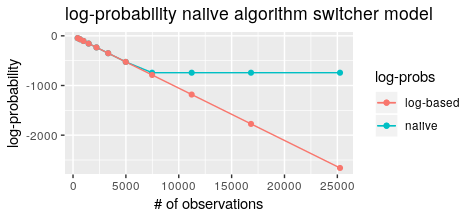
\includegraphics[width=\linewidth]{../forward_algorithm/superiority_log_approach.png}
	\caption{The log probability of the naiive implementation deviates from the result we would expect mathematically (straight line with constant negatie slope), but conforms to our prediction with assumed underflow. As expected, log implementation does not exhibit any deviation.}
	\label{log_impl_no_more_underflow}
\end{figure}


















